% !TeX root = ../build/main.tex

In the previous subsection, we explained how a user sends a ZKP onchain to use a license. In this process, the network validates that an unknown license has been used, and a session is opened. When the user communicates offchain with the SP, they provide a session cookie to verify that the session is opened onchain and the arguments are correct. One of these arguments, the attribute data $\attrdata$, is what defines the license (e.g., a ticket token, a set of personal information...), and this data is leaked to the SP. However, some use cases could require attribute data to be verified according to some conditions, for instance, leaking the information only partially. We now introduce a scheme to perform several attribute verifications offchain.

In our scheme, each SP decides which requirements the users need to meet, and provides a circuit that performs such checks. Then, when the user wants to use a service, will provide the session cookie as explained in the generic protocol, with the difference that \textbf{shall not include} the opening to $\com_1$. Instead, will provide a ZKP computed out of the circuit required by the SP. For this to work, an agreement between the different involved parties is needed, i.e. both LPs and SPs will need to agree on the language (or encoding) used to create the attributes of the license. In such regard, the value $\attrdata$ used in the license becomes the hash of some specific attributes, as follows:

$$\attrdata = \hp(\attr_0, \attr_1, ..., \attr_N, r_\mathsf{attr}),$$

where $r_\mathsf{attr}$ has to be a random value known by the user and the LP. For instance, the public key stored in their ID card.\\

The SP will accept the service if the user provides a valid session cookie and a valid proof out of the following sample circuit, where the value $\com_1$ included in the public inputs must be equal to the value $\Session.\com_1$:

\begin{figure}[H]
	\centering
	\setlength{\fboxsep}{5pt}%
	\setlength{\fboxrule}{0.3pt}%
	\fbox{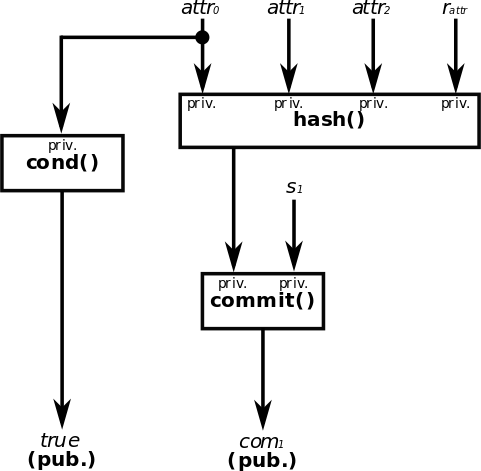
\includegraphics[width=140pt,draft=false]{\figs/circuit-offchain.png}}
	\caption{Arithmetic circuit for proving attributes off-chain.}
	\label{fig:circuit-offchain}
\end{figure}

\vspace{-0.3cm}
The above circuit from Figure~\ref{fig:circuit-offchain} can include as many conditions as desired for the attributes.